
\section{Empirical Test}\label{sec:empirical}
This section tests the pair-level prediction attached to Corollary~\ref{cor:copula-fail} and Remark~\ref{rem:small-cases}: across a wall the induced correlation jump $\Deltait_R$ of \eqref{eq:corr-jump} is positive on pairs whose two coins both lie in the wall-affected block, of opposite sign on pairs with exactly one coin in the block, and zero on pairs with neither. The panel is the \NPANEL-stablecoin archival panel across the \NEVENTS\ documented de-peg episodes of Table~\ref{tab:events}; the test statistic is a difference-in-differences across pair layers, introduced in \S\ref{sec:gradient} and estimated on the primary event in \S\ref{sec:usdc-svb}.

\subsection{Panel, dating, and the observable}\label{sec:panel}
The panel is the \NPANEL\ stablecoins listed in Appendix~\ref{app:data}, spanning four tiers (fiat-backed, crypto-collateralized, algorithmic, RWA/multi-asset). Daily peg deviations are taken from the DeFiLlama public archive over 2020--2025 and cross-checked against Chainlink oracle feeds and CoinGecko quotations; no proprietary or issuer-internal data is used. Each event is dated by the primary structural failure identified in the regulator and post-mortem literature (Appendix~\ref{app:data}). The wall assignment in the historical record draws on post-mortem accounts. In live use the channel is identified by the failure event itself, which is observable as it happens. The diagnostic is therefore a monitor of a channel's incidence rather than a forecast of its onset, and its value lies in telling a supervisor which coins a channel has already reached. The \emph{pre}-event window is the 60 calendar days preceding the event, trimmed to observations with non-missing prices (typically 46 trading days); the \emph{acute} window is the eleven calendar days centred on the event. Because the acute window is centred, it contains days on both sides of the crossing, which pulls $\rho^+$ back toward $\rho^-$ and biases $\Delta\rho$ toward zero rather than away from it: the test is conservative in this respect, and \S\ref{sec:robust} reports how the result moves as the acute width is varied. Both windows are used only to compute correlations; no pre-window observation enters the definition of the wall-affected block $B_W$, which is fixed ex ante from the wall taxonomy (Assumption~\ref{ass:support}).

\paragraph{The observable.} For each event and each pair of coins $(i,j)$ with at least five usable observations in each window, write $\rho^-_{ij}$ for the Pearson correlation of daily peg deviations over the pre-window and $\rho^+_{ij}$ for the acute window, and set
\begin{equation}\label{eq:delta-rho}
\Delta\rho_{ij} := \rho^+_{ij} - \rho^-_{ij}.
\end{equation}
This is the empirical counterpart of the entry $\Deltait_R{}_{ij}$ of the induced correlation jump \eqref{eq:corr-jump}: the pre-window estimates the chamber value $\Sigmait^-$, the acute window estimates the post-crossing value $\Sigmait^+$, and the difference estimates the jump. The identification of a pre-event window with a chamber requires two things of that window: that it be long enough for the peg-deviation law to settle inside the pre-crossing regime, and that it be short enough to precede the event. The first is examinable through the window grid of \S\ref{sec:robust}, which varies the pre-window between 30 and 90 days; the second we take as given, since the acute window is defined around the event date and the pre-window ends before it begins. Two properties of the theory are deliberately \emph{not} used as targets, because the normalisation map cannot deliver them: the jump is not claimed to be rank-one in correlation space, and its magnitude in correlation units is not claimed to be portable across events. What the theory does deliver---Corollary~\ref{cor:wall-jump} and Remark~\ref{rem:small-cases}---is the signed three-tier footprint of the jump: positive on block pairs, opposite-signed on cross pairs, zero outside. Those are the objects tested, and the test is stated on the block layer, whose sign the theory fixes without reference to the relative scale of the other two.

\subsection{The pair-level gradient test}\label{sec:gradient}
Classify each pair by how many of its two coins lie in the wall-affected block $B$ of the event:
\begin{itemize}[leftmargin=1.6em,itemsep=1pt]
\item \textbf{BLOCK}: both coins in $B$;
\item \textbf{CROSS}: exactly one coin in $B$;
\item \textbf{OUTSIDE}: neither coin in $B$.
\end{itemize}
Remark~\ref{rem:small-cases} fixes the sign of each layer and the size ordering between them, and it leaves one comparison open. The jump is positive on BLOCK pairs and zero on OUTSIDE pairs, whose two diagonals are untouched; on CROSS pairs it is opposite-signed and an order smaller in $a$, so the theory does not rank CROSS against OUTSIDE at first order. The substantive, testable claim is therefore that the block layer stands above both others:
\begin{equation}\label{eq:gradient-prediction}
\overline{\Delta\rho}_{\mathrm{BLOCK}} \;>\; \overline{\Delta\rho}_{\mathrm{CROSS}}
\quad\text{and}\quad
\overline{\Delta\rho}_{\mathrm{BLOCK}} \;>\; \overline{\Delta\rho}_{\mathrm{OUTSIDE}},
\end{equation}
where bars denote means within layer. The pure crossing law does place CROSS \emph{below} OUTSIDE, since the cross-pair image is opposite-signed (Remark~\ref{rem:small-cases}); but the observed level of every layer is contaminated by crisis-wide co-movement in proportions this design cannot separate, so the CROSS-versus-OUTSIDE ranking is reported as an empirical quantity and is not used as a test. The tested claim is the block-versus-rest contrast.

\paragraph{Why the comparison is a difference-in-differences.} A crisis of the kind in Table~\ref{tab:events} raises co-movement across the whole panel, not only inside the block. That common component enters every layer and is removed by the leading difference in \eqref{eq:gradient-prediction}: the estimate
\begin{equation}\label{eq:did}
\widehat{\mathrm{DiD}} := \overline{\Delta\rho}_{\mathrm{BLOCK}} - \overline{\Delta\rho}_{\mathrm{BLOCK}^{\mathsf{c}}}
\end{equation}
isolates the excess co-movement of block pairs over all other pairs. A smooth-surface model with no block structure predicts $\widehat{\mathrm{DiD}} = 0$; a model in which the entire effect is a single-coin (victim) shock predicts it only through pairs containing the victim, which is tested directly in \S\ref{sec:usdc-svb}.

The subtraction carries an identifying condition, which we state explicitly. Assumption~\ref{ass:support} implies that pairs outside the block carry no crossing contribution at all, so the theory predicts a \emph{zero} OUTSIDE layer; the observed OUTSIDE means are not zero (Table~\ref{tab:gradient}). A component the theory does not model is therefore present, and $\widehat{\mathrm{DiD}}$ identifies the block effect only if that component is additive and does not differ systematically across layers. We adopt that as an explicit identifying condition, not as a consequence of the theory, and \S\ref{sec:usdc-svb} reports the OUTSIDE level so that a reader can see how much of the raw co-movement the subtraction is absorbing.

\paragraph{Inference.} Pairs share coins and are therefore not independent, so the pair-level permutation test that treats pairs as exchangeable overstates precision. The primary inference is accordingly a \emph{coin-level} permutation: the block label is redrawn over sets of coins of the same size as $B$, and $\widehat{\mathrm{DiD}}$ recomputed, holding the pair-level statistic fixed. This asks the right question---how unusual is the true block among the $\binom{n}{|B|}$ coin sets that could have been labelled a block---and it is the test reported throughout. Pair-level permutation is reported alongside it as the (anti-conservative) comparison. A coin-level bootstrap interval is also reported. It is conditional on the block assignment, so it measures the sampling variability of coins under that assignment rather than the distinctiveness of the block itself, which is what the permutation test supplies.

\paragraph{Domain of the test.}\label{sec:single} The gradient requires a wall-affected block of at least two coins, so that a BLOCK pair exists at all. Six of the nine events in Table~\ref{tab:events} (UST/LUNA, USDT, BUSD, USDe, GHO, and DAI Black Thursday) have single-coin blocks, for which $\mathrm{BLOCK} = \emptyset$ and the criterion \eqref{eq:gradient-prediction} is undefined. They are outside the design and no statistic is reported for them.

\subsection{Primary event: the USDC--SVB weekend}\label{sec:usdc-svb}
The primary event is the USDC custody shock of 10--13 March 2023, which crosses three walls (Table~\ref{tab:events}). The block tested is the union of the three walls' blocks, fixed ex ante from the taxonomy, namely $\{\text{USDC},\text{DAI},\text{FRAX}\}$. For a single-wall event the tested block and the wall's block coincide; for this event the prediction is the union, which is what Assumption~\ref{ass:support} applied wall by wall delivers. The panel supplies \GUSDCSVBNB\ BLOCK pairs, \GUSDCSVBNC\ CROSS pairs and \GUSDCSVBNO\ OUTSIDE pairs.

\begin{table}[!ht]
\centering
\caption{Pair-level gradient on the three events that carry a multi-coin wall-affected block. Entries are layer means of $\Delta\rho$, the change in peg-deviation correlation from the 60-day pre-window to the acute window \eqref{eq:delta-rho}, with pair counts in parentheses; layers are defined in \S\ref{sec:gradient}. $\widehat{\mathrm{DiD}}$ is the block-versus-rest contrast \eqref{eq:did}. $p_{\text{coin}}$ is the coin-level permutation (the operative test), $p_{\text{pair}}$ the pair-level permutation reported for comparison; both are one-sided against the no-block null.}
\label{tab:gradient}
\begin{tabular}{@{}lrrrrrr@{}}
\toprule
& BLOCK & CROSS & OUTSIDE & $\widehat{\mathrm{DiD}}$ & $p_{\text{coin}}$ & $p_{\text{pair}}$ \\
\midrule
USDC--SVB & $\GUSDCSVBB$ (\GUSDCSVBNB) & $\GUSDCSVBC$ (\GUSDCSVBNC) & $\GUSDCSVBO$ (\GUSDCSVBNO) & $\GUSDCSVBDID$ & $\GUSDCSVBPCOIN$ & $\GUSDCSVBPPAIR$ \\
FTX       & $\GFTXB$ (\GFTXNB) & $\GFTXC$ (\GFTXNC) & $\GFTXO$ (\GFTXNO) & $\GFTXDID$ & $\GFTXPCOIN$ & $\GFTXPPAIR$ \\
FDUSD     & $\GFDUSDB$ (\GFDUSDNB) & $\GFDUSDC$ (\GFDUSDNC) & $\GFDUSDO$ (\GFDUSDNO) & $\GFDUSDDID$ & $\GFDUSDPCOIN$ & $\GFDUSDPPAIR$ \\
\bottomrule
\end{tabular}
\end{table}

The prediction \eqref{eq:gradient-prediction} holds: BLOCK $= \GUSDCSVBB$ (Table~\ref{tab:gradient}, Figure~\ref{fig:gradient}a) stands above both CROSS $= \GUSDCSVBC$ and OUTSIDE $= \GUSDCSVBO$, by a factor of two or more against either. The difference-in-differences is $\widehat{\mathrm{DiD}} = \GUSDCSVBDID$, and the coin-level permutation leaves the true block above \GUSDCSVBPCT\% of the 816 candidate coin sets ($p = \GUSDCSVBPCOIN$). The pair-level test, which treats pairs as exchangeable, gives $p = \GUSDCSVBPPAIR$; the two agree in conclusion, and we report the coin-level figure as the operative one.

\begin{figure}[!ht]
\centering
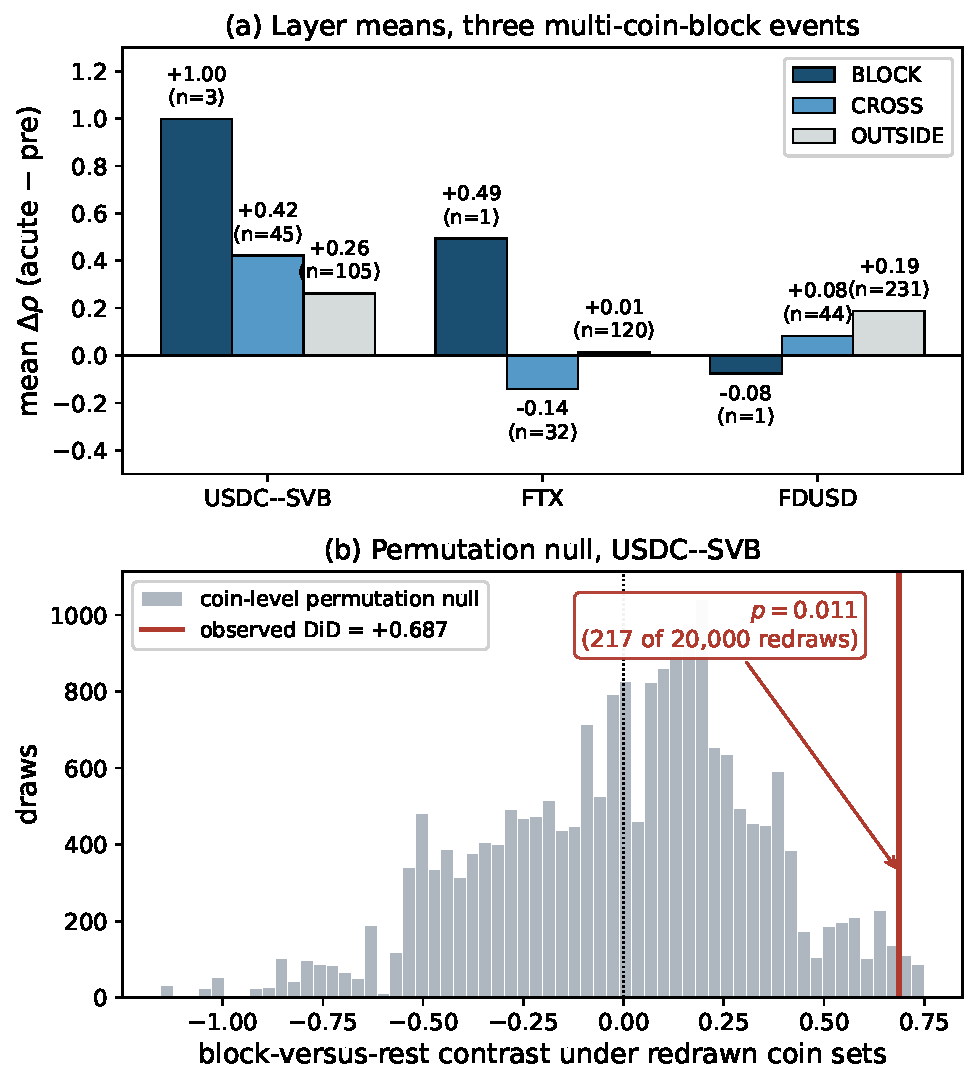
\includegraphics[width=0.9\textwidth]{figs/fig2_gradient}
\caption{The pair-level gradient test. (a) Mean change in peg-deviation correlation $\Delta\rho$ by pair layer for the three events with a multi-coin wall-affected block, with pair counts in parentheses. The criterion \eqref{eq:gradient-prediction} holds on USDC--SVB and on FTX, and fails on FDUSD, where the BLOCK bar sits below both other layers. (b) The coin-level permutation null for the primary event: block labels are redrawn over sets of three coins and the block-versus-rest contrast recomputed for each of 20{,}000 draws. The observed contrast sits in the upper tail.}
\label{fig:gradient}
\end{figure}

This is the block signature of the primary event, read off an acute-window correlation submatrix. Everything it requires is a public price series: no proprietary data, no issuer disclosure, and no estimation of the crossing amplitude. A supervisor can compute it on the same panel, and \S\ref{sec:robust} reports how it behaves when the window is moved.

\paragraph{The block effect is not a victim effect.} Two of the three BLOCK pairs contain USDC, the primary victim, so a sceptical reading would attribute the gradient to victim membership rather than to block membership. The test against that reading is the remaining pair. The pair $(\text{DAI},\text{FRAX})$ tests that reading. Neither coin held reserves at SVB: both enter the block through the transmission channel $W_1$ rather than through the custody channel $W_4$, because DAI was partly backed by USDC and FRAX held USDC among its collateral. Their block membership is therefore fixed by the wall taxonomy and not by the outcome. Their jump is $\GUSDCSVBPURE$, larger than the BLOCK mean itself. A victim-only account predicts no jump on this pair; the block account predicts one, and the realised value is the largest in the panel. What the pair establishes is that the effect does not require the coin that actually failed---not that no common exposure is involved, since the shared USDC collateral is precisely what put both coins in the block.

\paragraph{What the OUTSIDE layer shows.} The theory says this layer should not move, and it does: the OUTSIDE mean is $\GUSDCSVBO$, positive and substantial. That is the component of \S\ref{sec:gradient} which the theory does not model and which the block-versus-rest contrast is designed to absorb. The theory's content is therefore the excess of BLOCK over that baseline, $\GUSDCSVBDID$, not the level of either---and the contrast is only as good as the identifying condition stated there.

\subsection{Two secondary events}\label{sec:ftx-fdusd}
The remaining two multi-coin-block events supply one BLOCK pair each, so their layer means rest on a single observation (Table~\ref{tab:gradient}, rows two and three).

\paragraph{FTX contagion (November 2022).} The wall-affected block is $\{\text{USDD},\text{MIM}\}$, two coins with material Alameda/FTX counterparty exposure. BLOCK $= \GFTXB$ stands above both OUTSIDE $= \GFTXO$ and CROSS $= \GFTXC$, giving $\widehat{\mathrm{DiD}} = \GFTXDID$; the true block sits above \GFTXPCT\% of the $\binom{18}{2}$ alternative coin pairs, with $p = \GFTXPCOIN$. The criterion \eqref{eq:gradient-prediction} holds under eight of the nine window specifications, the exception being the 30-day pre-window with a $\pm10$-day acute window (Table~\ref{tab:robust}). A single BLOCK pair is one draw against the alternatives, so the permutation bounds what this event can resolve.

\paragraph{FDUSD 2024 (November 2024).} The block is $\{\text{FDUSD},\text{TUSD}\}$, again a single BLOCK pair, and here BLOCK $= \GFDUSDB$ lies below OUTSIDE $= \GFDUSDO$, giving $\widehat{\mathrm{DiD}} = \GFDUSDDID$ and $p = \GFDUSDPCOIN$. The criterion \eqref{eq:gradient-prediction} holds only under a 30-day pre-window and fails under the 60- and 90-day windows (Table~\ref{tab:robust}). Its wall assignment $W_3+W_2$ places the episode in the gate/oracle family rather than the custody family, and the episode is of low intensity.

\subsection{Robustness and scope}\label{sec:robust}
\paragraph{Inference.} The conclusion for the primary event is unchanged between the pair-level permutation ($p = \GUSDCSVBPPAIR$) and the coin-level permutation ($p = \GUSDCSVBPCOIN$). The coin-level bootstrap interval for $\widehat{\mathrm{DiD}}$ is $[\GUSDCSVBLO,\ \GUSDCSVBHI]$; it excludes zero, but as noted in \S\ref{sec:gradient} it is conditional on the block assignment and does not test block distinctiveness, which is why the permutation test carries the inference.

\paragraph{Window and threshold.} The window specification enters only through $\rho^-$ and $\rho^+$. The full $3 \times 3$ grid---pre-window of 30, 60 or 90 days crossed with an acute half-width of $\pm3$, $\pm5$ or $\pm10$ days---leaves both the sign and the criterion \eqref{eq:gradient-prediction} unchanged on the primary event, with $\widehat{\mathrm{DiD}}$ ranging over $[0.58, 0.79]$ against the canonical $\GUSDCSVBDID$ (Table~\ref{tab:robust} in Appendix~\ref{app:oos}). The same grid is reported there for the two secondary events, where it also documents the intermediate-step violation on FTX and the window-dependence of the FDUSD sign disclosed above.

\paragraph{Composition of the event record.} Three of the nine events carry a multi-coin block, and two of those supply a single BLOCK pair (Table~\ref{tab:gradient}). De-peg episodes with a multi-coin block are rare by nature, so the sample is bounded by the 2020--2025 record rather than by any selection on outcomes.
